\def\sectiontitle{Conclusion}

\section{\sectiontitle}

%%%%%%%%%%%%%%%%%%%%%%%%%%%%%%%%%%%%%%%%%%%%%%%%%%%%%%%%%%%%%%%%%%%%%%%%%%%%%%%%
\def\slidetitle{New WIPP plugins}

\subsection{\slidetitle}
\begin{frame}
  \frametitle{\sectiontitle}
  \framesubtitle{\slidetitle}

  Inference plugins
  \begin{itemize}
    \item Hugging Face:
    \item BioImage.IO:
    \item SAM2: 
    \item Cellpose: 
  \end{itemize}

  Accuracy plugin
  \begin{itemize}
    \item Dice: 
  \end{itemize}

\end{frame}

%%%%%%%%%%%%%%%%%%%%%%%%%%%%%%%%%%%%%%%%%%%%%%%%%%%%%%%%%%%%%%%%%%%%%%%%%%%%%%%%
\def\slidetitle{Fine-tuning plugin}

\subsection{\slidetitle}
\begin{frame}
  \frametitle{\sectiontitle}
  \framesubtitle{\slidetitle}

  \begin{minipage}[h!]{0.53\textwidth}
    Goal
    \begin{itemize}
      \item Improve already existing AI models
    \end{itemize}

    \bigskip

    Work
    \begin{itemize}
      \item Identify if models can be retrain/fine-tune
      \item Plugin to fine-tune an AI model
    \end{itemize}

  \end{minipage}\hfill
  \begin{minipage}[h!]{0.46\textwidth}
    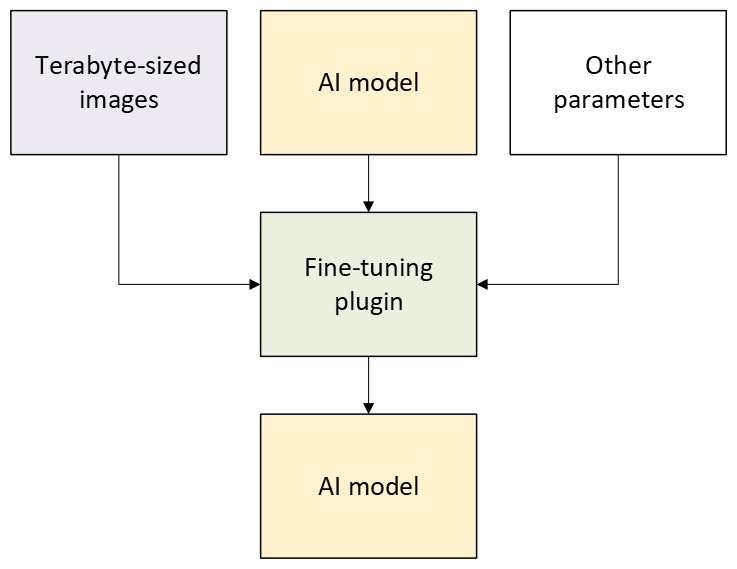
\includegraphics[scale=0.55]{./img/5_conclusion.png}
  \end{minipage}
\end{frame}